% !TEX program = xelatex
\documentclass[a4paper,UTF8]{ctexart}
\usepackage[unicode=true,colorlinks,urlcolor=blue,linkcolor=blue,bookmarksnumbered=true]{hyperref}
\usepackage{latexsym,amssymb,amsmath,amsbsy,amsopn,amstext,amsthm,amsxtra,mathrsfs,color,multicol,bm,calc,ifpdf}
\usepackage{graphicx}
\usepackage{diagbox}   % 绘制表格斜线
\usepackage{enumerate}
\usepackage{epstopdf}
\usepackage{tikz}
\usetikzlibrary{calc}
\usepackage{fancyhdr}
\usepackage{subfigure}
\usepackage{listings}
\usepackage{multirow}
\usepackage{makeidx}
\usepackage{tabularx}
\usepackage{xcolor} 
\usepackage{fontspec}                            % 建立索引宏包
\graphicspath{{figures/}}  % 设置图片搜索路径
\theoremstyle{plain} \newtheorem{theorem}{定理}[section]
\theoremstyle{plain} \newtheorem{definition}{定义}[section]
\theoremstyle{plain} \newtheorem{lemma}{引理}[section]
\theoremstyle{plain} \newtheorem{proposition}{命题}[section]
\theoremstyle{plain} \newtheorem{example}{例}
\theoremstyle{plain} \newtheorem{remark}{注}
\theoremstyle{plain} \newtheorem{corollary}{推论}[section]
\newfontfamily\courier{Courier New}
\lstset{linewidth=1.1\textwidth,
        numbers=left, %设置行号位置 
        basicstyle=\small\courier,
        numberstyle=\tiny\courier, %设置行号大小  
        keywordstyle=\color{blue}\courier, %设置关键字颜色  
        %identifierstyle=\bf,
        commentstyle=\it\color[cmyk]{1,0,1,0}\courier, %设置注释颜色 
        stringstyle=\it\color[RGB]{128,0,0}\courier,
        %framexleftmargin=10mm,
        frame=single, %设置边框格式  
        backgroundcolor=\color[RGB]{245,245,244},
        %escapeinside=``, %逃逸字符(1左面的键),用于显示中文  
        breaklines, %自动折行  
        extendedchars=false, %解决代码跨页时,章节标题,页眉等汉字不显示的问题  
        xleftmargin=2em,xrightmargin=2em, aboveskip=1em, %设置边距  
        tabsize=4, %设置tab空格数  
        showspaces=false %不显示空格  
        basicstyle=\small\courier
       }  
\newenvironment{mysolution}{{\color{blue} 解}: }{{\color{magenta}\qed}}
\newcommand\diff{\,{\mathrm d}} %定义微分d
\newcommand{\p}[3]{\frac{\partial^{#1}#2}{\partial{#3}^{#1}}}  %定义求偏导算子
\newcommand{\ucite}[1]{\textsuperscript{\cite{#1}}}  %参考文献引用:上标用\ucite{ },文中用\cite{ }

\begin{document}
\title{

\includegraphics[width=0.65\textwidth]{onepiece.pdf}\\
\vspace{2em}
\textbf{决策树学习笔记}}
\author{\emph{李向阳} \quad {\color{blue} d1142845997@gmail.com}
}
\date{}


\maketitle
\thispagestyle{empty}

\newpage


\tableofcontents

\newpage

\section{引入}
决策树主要有两种, 一种是分类树, 一种是回归树, 这里主要讨论分类树, 并顺带会提及回归树.

我们用$\bm{x} = (x_{1}, x_{2}, \cdots, x_{n})^{T}$表示样本的$n$个特征(features), 注意特征的取值可以是连续的, 也可以是离散的, 用$y$表示样本的类别, 假设有$K$类, 用$y = k$表示样本属于第$k$类, $k = 1, 2, \cdots, K$, 即$y \in \{ 1, 2, \cdots, K \}$. 假设现在我们有$m$个训练样本, 即$\{\bm{x}^{(i)}, y^{(i)}\}, i = 1, 2, \cdots, m$, 很多文献中把样本实例也称作“特征向量”(feature vertor), 其中
\begin{equation*}
\bm{x}^{(i)} = (x_{1}^{(i)}, x_{2}^{(i)}, \cdots, x_{n}^{(i)})^{T},i = 1, 2, \cdots, m
\end{equation*}

我们的的目标是根据给定的训练数据集构建一个决策树模型, 使它能够对实例进行正确的分类.

\section{三个经典例子}
\subsection{信贷的例子}
\begin{example}
我们希望能够学习出一个贷款申请的决策树, 当新的客户提出申请贷款时, 根据申请人的特征利用决策树决定是否批准申请贷款.

\begin{table}[!htb]
\centering
\caption{信贷数据}
\label{xindai}
\begin{tabular}{cccccc}
  \hline
    % after \: \hline or \cline{col1-col2} \cline{col3-col4} ...
    \textbf{ID} & \textbf{年龄} & \textbf{有工作} & \textbf{有自己的房子} & \textbf{信贷情况} & \textbf{类别}\\
    \hline
    1 & 青年 & 否 & 否 &  一般  & 否 \\
    \hline
    2 & 青年 & 否 & 否 &  好  & 否 \\
    \hline
    3 & 青年 & 是 & 否 &  好  & 是 \\
    \hline
    4 & 青年 & 是 & 是 &  一般  & 是 \\
    \hline
    5 & 青年 & 否 & 否 &  一般  & 否 \\
    \hline
    6 & 中年 & 否 & 否 &  一般  & 否 \\
    \hline
    7 & 中年 & 否 & 否 &  好  & 否 \\
    \hline
    8 & 中年 & 是 & 是 &  好  & 是 \\
    \hline
    9 & 中年 & 否 & 是 &  非常好  & 是 \\
    \hline
    10 & 中年 & 否 & 是 &  非常好  & 是 \\
    \hline
    11 & 老年 & 否 & 是 &  非常好  & 是 \\
    \hline
    12 & 老年 & 否 & 是 &  好  & 是 \\
    \hline
    13 & 老年 & 是 & 否 &  好  & 是 \\
    \hline
    14 & 老年 & 是 & 否 &  非常好  & 是 \\
    \hline
    15 & 老年 & 否 & 否 &  一般  & 否 \\

  \hline
\end{tabular}
\end{table}

\end{example}

虽然这也是一个二分类问题, 但是用 Logistic 回归之类的方法就不太能行得通了. 我们来构建决策树模型.

在这个例子中, 样本集合$D$总共有$4$个特征, 分别是年龄, 工作, 房子和信贷情况, 它们取值如下:
\begin{table}[!htb]
\centering
\caption{信贷特征取值}
\label{xindaivalue}
\begin{tabularx}{10cm}{XX}
  \hline
    % after \: \hline or \cline{col1-col2} \cline{col3-col4} ...
    \textbf{特征} & \textbf{取值}  \\
    \hline
    年龄   &  青年,中年,老年 \\
    \hline
    工作   &  是,否 \\
    \hline
    房子   &  是,否 \\
    \hline
    信贷情况   &  一般,好,非常好 \\
  \hline
\end{tabularx}
\end{table}

如果我们根据这些条件逐步去构建决策树的话, 如何选择每个节点呢? 比如我们的根节点是选年龄好还是选工作好? 不同的算法选择的标准不一样. 下面介绍 ID3(Iterative Dichotomiser)算法.

ID3 算法根据信息增益(Information Gain)来选取特征作为决策树分裂的节点. 特征$A$对训练数据集$D$的信息增益定义为集合$D$的经验熵(所谓经验熵, 指的是熵是由某个数据集合估计得到的)$H(D)$与特征$A$给定条件下$D$的经验条件熵$H(D∣A)$之差, 记为$g(D, A)$.
\begin{equation*}
g(D, A) = H(D) - H(D | A)
\end{equation*}

这实际上就是特征$A$和$D$的互信息. 我们分别以$A_1, A_2, A_3, A_4$来表示年龄, 工作, 房子和信贷情况这$4$个特征. 下面就来计算每个特征的信息增益.

为了方便叙述, 我们将类别为是的类标记为正类, 类别为否的类标记为负类, 那么$15$个样本中有$9$个是正类, $6$个是负类, 因此数据集$D$的经验熵为
\begin{equation*}
H(D) = - \frac{9}{15} \log \frac{9}{15} - \frac{6}{15} \log \frac{6}{15} = 0.971
\end{equation*}

注意这里的对数以$2$为底.

接下来我们先计算$g(D, A_{1}) = H(D) - H(D | A_{1})$, 而
\begin{equation}\label{age}
H(D|A_{1}) = \frac{5}{15} H(D|A_{1} = \textrm{青年}) + \frac{5}{15} H(D|A_{1} = \textrm{中年}) + \frac{5}{15} H(D|A_{1} = \textrm{老年})
\end{equation}

当$A_{1} = \textrm{青年}$时, 即观察青年人中, 共有$5$个人, 其中 2 个是正类, 3 个是负类, 因此
\begin{equation*}
H(D|A_{1} = \textrm{青年}) = - \frac{2}{5} \log \frac{2}{5} - \frac{3}{5} \log \frac{3}{5} = 0.971
\end{equation*}

当$A_{1} = \textrm{中年}$时, 即观察中年人中, 共有$5$个人,其中 3 个是正类, 2 个是负类, 因此
\begin{equation*}
H(D | A_{1} = \textrm{中年}) = - \frac{3}{5} \log \frac{3}{5} - \frac{2}{5} \log \frac{2}{5} = 0.971
\end{equation*}

当$A_{1} = \textrm{老年}$时, 即观察老年人中, 共有$5$个人,其中 4 个是正类, 1 个是负类, 因此
\begin{equation*}
H(D | A_{1} = \textrm{老年}) = - \frac{4}{5} \log \frac{4}{5} - \frac{1}{5} \log \frac{1}{5} = 0.722
\end{equation*}

把结果代入到(\ref{age})中, 可得
\begin{equation*}
H(D | A_{1}) = \frac{5}{15} \times 0.971 + \frac{5}{15} \times 0.971 + \frac{5}{15} \times 0.722 = 0.888
\end{equation*}

于是可得
\begin{equation*}
g(D, A_{1}) = H(D) - H(D | A_{1}) = 0.971 - 0.888 = 0.083
\end{equation*}

把上述过程写的紧凑一点, 也即
\begin{align*}
g(D, A_{1}) & = H(D) - \left[ \frac{5}{15} H(D_{1}) + \frac{5}{15} H(D_{2}) + \frac{5}{15} H(D_{3}) \right] \\ 
& = 0.971 - \left[ \frac{5}{15} \left( - \frac{2}{5} \log \frac{2}{5} - \frac{3}{5} \log \frac{3}{5} \right) \right. \\ 
& \quad + \left. \frac{5}{15} \left( - \frac{3}{5} \log \frac{3}{5} - \frac{2}{5} \log \frac{2}{5} \right) + \frac{5}{15} \left( - \frac{4}{5} \log \frac{4}{5} - \frac{1}{5} \log \frac{1}{5} \right) \right] \\ 
& = 0.971 - 0.888 = 0.083
\end{align*}

其中$D_{1}, D_{2}, D_{3}$分别是$D$中$A_{1}$(年龄)取值为青年、中年和老年的样本子集.

同理可得
\begin{align*}
g(D, A_{2}) & = H(D) - \left[ \frac{5}{15} H(D_{1}) + \frac{10}{15} H(D_{2}) \right] \\ 
& = 0.971 - \left[ \frac{5}{15} \times 0 + \frac{10}{15} \left( - \frac{4}{10} \log \frac{4}{10} - \frac{6}{10} \log \frac{6}{10}  \right) \right] = 0.324 \\ 
g(D,A_{3}) & = H(D) - \left[ \frac{6}{15} H(D_{1}) + \frac{9}{15} H(D_{2}) \right] \\ 
& = 0.971 - \left[ \frac{6}{15} \times 0 + \frac{9}{15} \left( - \frac{3}{9} \log \frac{3}{9} - \frac{6}{9} \log \frac{6}{9}  \right) \right] = 0.420 \\ 
g(D,A_{4}) & = H(D) - \left[ \frac{5}{15} H(D_{1}) + \frac{6}{15} H(D_{2} + \frac{4}{15} H(D_{3} \right] \\ 
& = 0.971 - \left[ \frac{5}{15} \left( - \frac{1}{5} \log \frac{1}{5} - \frac{4}{5} \log \frac{4}{5} \right) \right. \\ 
& \quad + \left. \frac{6}{15} \left( - \frac{4}{6} \log \frac{4}{6} - \frac{2}{6} \log \frac{2}{6} \right) + \frac{4}{15} \times 0 \right] \\ 
& = 0.971 - 0.608 = 0.363
\end{align*}

由于$A_{3}$的信息增益最大, 所以选择特征$A_{3}$(有自己的房子)为最优特征, 即选为根节点. 它将数据集$D$划分为两个子集$D_{1}$($A_{3}$取值为“是”)和$D_{2}$($A_{3}$取值为“否”), 由于$D_{1}$只有同一类的样本点, 所以它成为一个叶节点, 节点的标记为“是”, 如下图所示:
\begin{figure}[!htb]
\centering
\begin{tikzpicture}[line width = 1pt]
\fill[blue] (0,0) circle (0.3);
\fill[blue] (2,-3) circle (0.3);
\fill[blue] (-2-0.3,-3-0.3) rectangle (-2+0.3,-3+0.3);  % 半径 r = 0.3
\draw[->] (0,-0.3) -- (2-0.2,-3+0.2);  % 粗略看出来的, 不精确
\draw[->] (0,-0.3) -- (-2,-3+0.3);
\node at(0,0.8){有自己的房子};
\node at(-1.3,-1.2){是};
\node at(1.2,-1.2){否};
\node at(-2.4,-3.6){是};
\end{tikzpicture}
\end{figure}


对于$D_{2}$, 则需从特征$A_{1}$(年龄), $A_{2}$(有工作)和$A_{4}$(信贷情况)中选择新的特征.

无房子的共有 9 人, 即集合$D_{2}$中有 9 人, 为了方便, 我们可以将表\ref{xindai}中这 9 个人再单独拿出来, 如下表:
\begin{table}[!htb]
\centering
\caption{无房子数据}
\label{house}
\begin{tabular}{cccccc}
  \hline
    % after \: \hline or \cline{col1-col2} \cline{col3-col4} ...
    \textbf{ID} & \textbf{年龄} & \textbf{有工作} & \textbf{有自己的房子} & \textbf{信贷情况} & \textbf{类别}\\
    \hline
    1 & 青年 & 否 & 否 &  一般  & 否 \\
    \hline
    2 & 青年 & 否 & 否 &  好  & 否 \\
    \hline
    3 & 青年 & 是 & 否 &  好  & 是 \\
    \hline
    5 & 青年 & 否 & 否 &  一般  & 否 \\
    \hline
    6 & 中年 & 否 & 否 &  一般  & 否 \\
    \hline
    7 & 中年 & 否 & 否 &  好  & 否 \\
    \hline
    13 & 老年 & 是 & 否 &  好  & 是 \\
    \hline
    14 & 老年 & 是 & 否 &  非常好  & 是 \\
    \hline
    15 & 老年 & 否 & 否 &  一般  & 否 \\

  \hline
\end{tabular}
\end{table}

其中有 3 个正类, 6 个负类, 因此$D_{2}$的经验熵为
\begin{equation*}
H(D_{2}) = - \frac{3}{9} \log \frac{3}{9} - \frac{6}{9} \log \frac{6}{9} = 0.918
\end{equation*}

进一步可得各个特征的信息增益为
\begin{align*}
g(D_{2},A_{1}) & = H(D_{2}) - H(D_{2} | A_{1}) \\ 
& = 0.918 - \left[ \frac{4}{9} \left( - \frac{1}{4} \log \frac{1}{4} - \frac{3}{4} \log \frac{3}{4} \right) + \frac{2}{9} \times 0 + \frac{3}{9} \left( - \frac{2}{3} \log \frac{2}{3} - \frac{1}{3} \log \frac{1}{3} \right) \right] \\ 
& = 0.918 - 0.667 = 0.251 \\ 
g(D_{2},A_{2}) & = H(D_{2}) - H(D_{2} | A_{2}) \\ 
& = 0.918 - \left[ \frac{3}{9} \times 0 + \frac{6}{9} \times 0 \right] \\ 
& = 0.918 - 0 = 0.918 \\ 
g(D_{2},A_{4}) & = H(D_{2}) - H(D_{2} | A_{4}) \\ 
& = 0.918 - \left[ \frac{4}{9} \times 0 + \frac{4}{9} \left( - \frac{2}{4} \log \frac{2}{4} - \frac{2}{4} \log \frac{2}{4} \right) + \frac{1}{9} \times 0 \right] \\ 
& = 0.918 - 0.444 = 0.474 
\end{align*}

这里$A_{2}$(有工作)的信息增益最大, 故选择$A_{2}$作为节点的特征, 它又将数据集$D_{2}$划分为两个部分, 即从这个节点又引出两个子节点, 一个对应“是”(有工作) 的子结点, 包含 3 个样本, 它们属于同一类, 所以这是一个叶结点, 类标记为“是”; 另一个是对应“否”(无工作)的子结点, 包含 6 个样本, 它们也属于同一类, 所以这也是一个叶结点, 类标记为“否”.

这样生成一个如下图\ref{xindaitree}所示的决策树. 该决策树只用到了两个特征(有两个内部结点).
\begin{figure}\label{xindaitree}
\centering
\begin{tikzpicture}[line width = 1pt]
\fill[blue] (0,0) circle (0.3);
\fill[blue] (2,-3) circle (0.3);
\fill[blue] (-2-0.3,-3-0.3) rectangle (-2+0.3,-3+0.3);  % 半径 r = 0.3
\fill[blue] (0-0.3,-6-0.3) rectangle (0+0.3,-6+0.3);
\fill[blue] (4-0.3,-6-0.3) rectangle (4+0.3,-6+0.3);
\draw[->] (0,-0.3) -- (2-0.2,-3+0.2);  % 粗略看出来的, 不精确
\draw[->] (0,-0.3) -- (-2,-3+0.3);
\draw[->] (2,-3-0.3) -- (0,-6+0.3);
\draw[->] (2,-3-0.3) -- (4,-6+0.3);
\node at(0,0.8){有自己的房子};
\node at(-1.3,-1.2){是};
\node at(1.2,-1.2){否};
\node at(-2,-3.6){是};
\node at(2+1.2,-3){有工作};
\node at(0.8,-4.2){是};
\node at(3.4,-4.2){否};
\node at(0,-6-0.6){是};
\node at(4,-6-0.6){否};
\end{tikzpicture}
\caption{决策树的生成}
\end{figure}




\subsection{打网球的例子}
数据集如下表:
\begin{table}[!htb]
\centering
\caption{网球数据}
\label{tennis}
\begin{tabular}{l|l|l|l|l|l}
  \hline
    % after \: \hline or \cline{col1-col2} \cline{col3-col4} ...
    \textbf{Day} & \textbf{Outlook} & \textbf{Temperature} & \textbf{Humidity} & \textbf{Wind} & \textbf{Play Tennis} \\
    \hline
    1 & Sunny & Hot & High & Weak & No \\ 
    \hline
    2 & Sunny & Hot & High & Strong  & No \\ 
    \hline
    3 & Overcast & Hot & High & Weak & Yes \\ 
    \hline 
    4 & Rain & Mild & High & Weak & Yes \\ 
    \hline
    5 & Rain & Cool & Normal & Weak & Yes \\ 
    \hline
    6 & Rain & Cool & Normal & Strong &  No \\ 
    \hline
    7 & Overcast & Cool & Normal & Strong & Yes \\ 
    \hline
    8 & Sunny & Mild & High & Weak & No \\ 
    \hline
    9 & Sunny & Cool & Normal & Weak & Yes \\ 
    \hline
    10 & Rain & Mild & Normal & Weak & Yes \\ 
    \hline
    11 & Sunny & Mild & Normal & Strong & Yes \\ 
    \hline
    12 & Overcast & Mild & High & Strong & Yes \\ 
    \hline
    13 & Overcast & Hot & Normal & Weak & Yes \\
    \hline
    14 & Rain & Mild & High & Strong & No \\ 
  \hline
\end{tabular}
\end{table}

数据集$D$中有 9 个正类, 5 个负类, 因此数据集$D$的经验熵为
\begin{equation*}
H(D) = - \frac{9}{14} \log \frac{9}{14} - \frac{5}{14} \log \frac{5}{14} = 0.940
\end{equation*}

采用与上例类似的符号, 我们用$A_{i}, i = 1,2,3,4$来表示样本的 4 个特征, 依次为 Outlook, Temperature, Humidity 和 Wind. 同样计算可得
\begin{align*}
g(D, A_{1}) & = H(D) - \left[ \frac{5}{14} H(D_{1}) + \frac{4}{14} H(D_{2}) + \frac{5}{14} H(D_{3}) \right] \\ 
& = 0.940 - \left[ \frac{5}{14} \left( - \frac{2}{5} \log \frac{2}{5} - \frac{3}{5} \log \frac{3}{5} \right) + \frac{4}{14} \times 0 + \frac{5}{14} \left( - \frac{3}{5} \log \frac{3}{5} - \frac{2}{5} \log \frac{2}{5} \right) \right] \\ 
& = 0.246
\end{align*}

\begin{align*}
g(D, A_{2}) & = H(D) - \left[ \frac{4}{14} H(D_{1}) + \frac{6}{14} H(D_{2}) + \frac{4}{14} H(D_{3}) \right] \\ 
& = 0.940 - \left[ \frac{4}{14} \left( - \frac{2}{4} \log \frac{2}{4} - \frac{2}{4} \log \frac{2}{4} \right) \right. \\ 
& \quad + \left. \frac{6}{14} \left( - \frac{4}{6} \log \frac{4}{6} - \frac{2}{6} \log \frac{2}{6} \right) + \frac{4}{14} \left( - \frac{3}{4} \log \frac{3}{4} - \frac{1}{4} \log \frac{1}{4} \right) \right] \\ 
& = 0.029 
\end{align*}

\begin{align*}
g(D, A_{3}) & = H(D) - \left[ \frac{7}{14} H(D_{1}) + \frac{7}{14} H(D_{2}) \right] \\ 
& = 0.940 - \left[ \frac{7}{14} \left( - \frac{3}{7} \log \frac{3}{7} - \frac{4}{7} \log \frac{4}{7} \right) + \frac{7}{14} \left( - \frac{6}{7} \log \frac{6}{7} - \frac{1}{7} \log \frac{1}{7} \right) \right] \\ 
& = 0.151 \\ 
g(D, A_{4}) & = H(D) - \left[ \frac{8}{14} H(D_{1}) + \frac{6}{14} H(D_{2}) \right] \\ 
& = 0.940 - \left[ \frac{8}{14} \left( - \frac{6}{8} \log \frac{6}{8} - \frac{2}{8} \log \frac{2}{8} \right) + \frac{6}{14} \left( - \frac{3}{6} \log \frac{3}{6} - \frac{3}{6} \log \frac{3}{6} \right) \right] \\ 
& = 0.048
\end{align*}

有的文献中用$S$表示集合, 用$Gain(S, A_{i})$表示特征$A_{i}$的增益, 上述计算过程可用下图表示(略去计算过程, 用图形展示更为直观).

\begin{figure}[!htb]
	\centering
	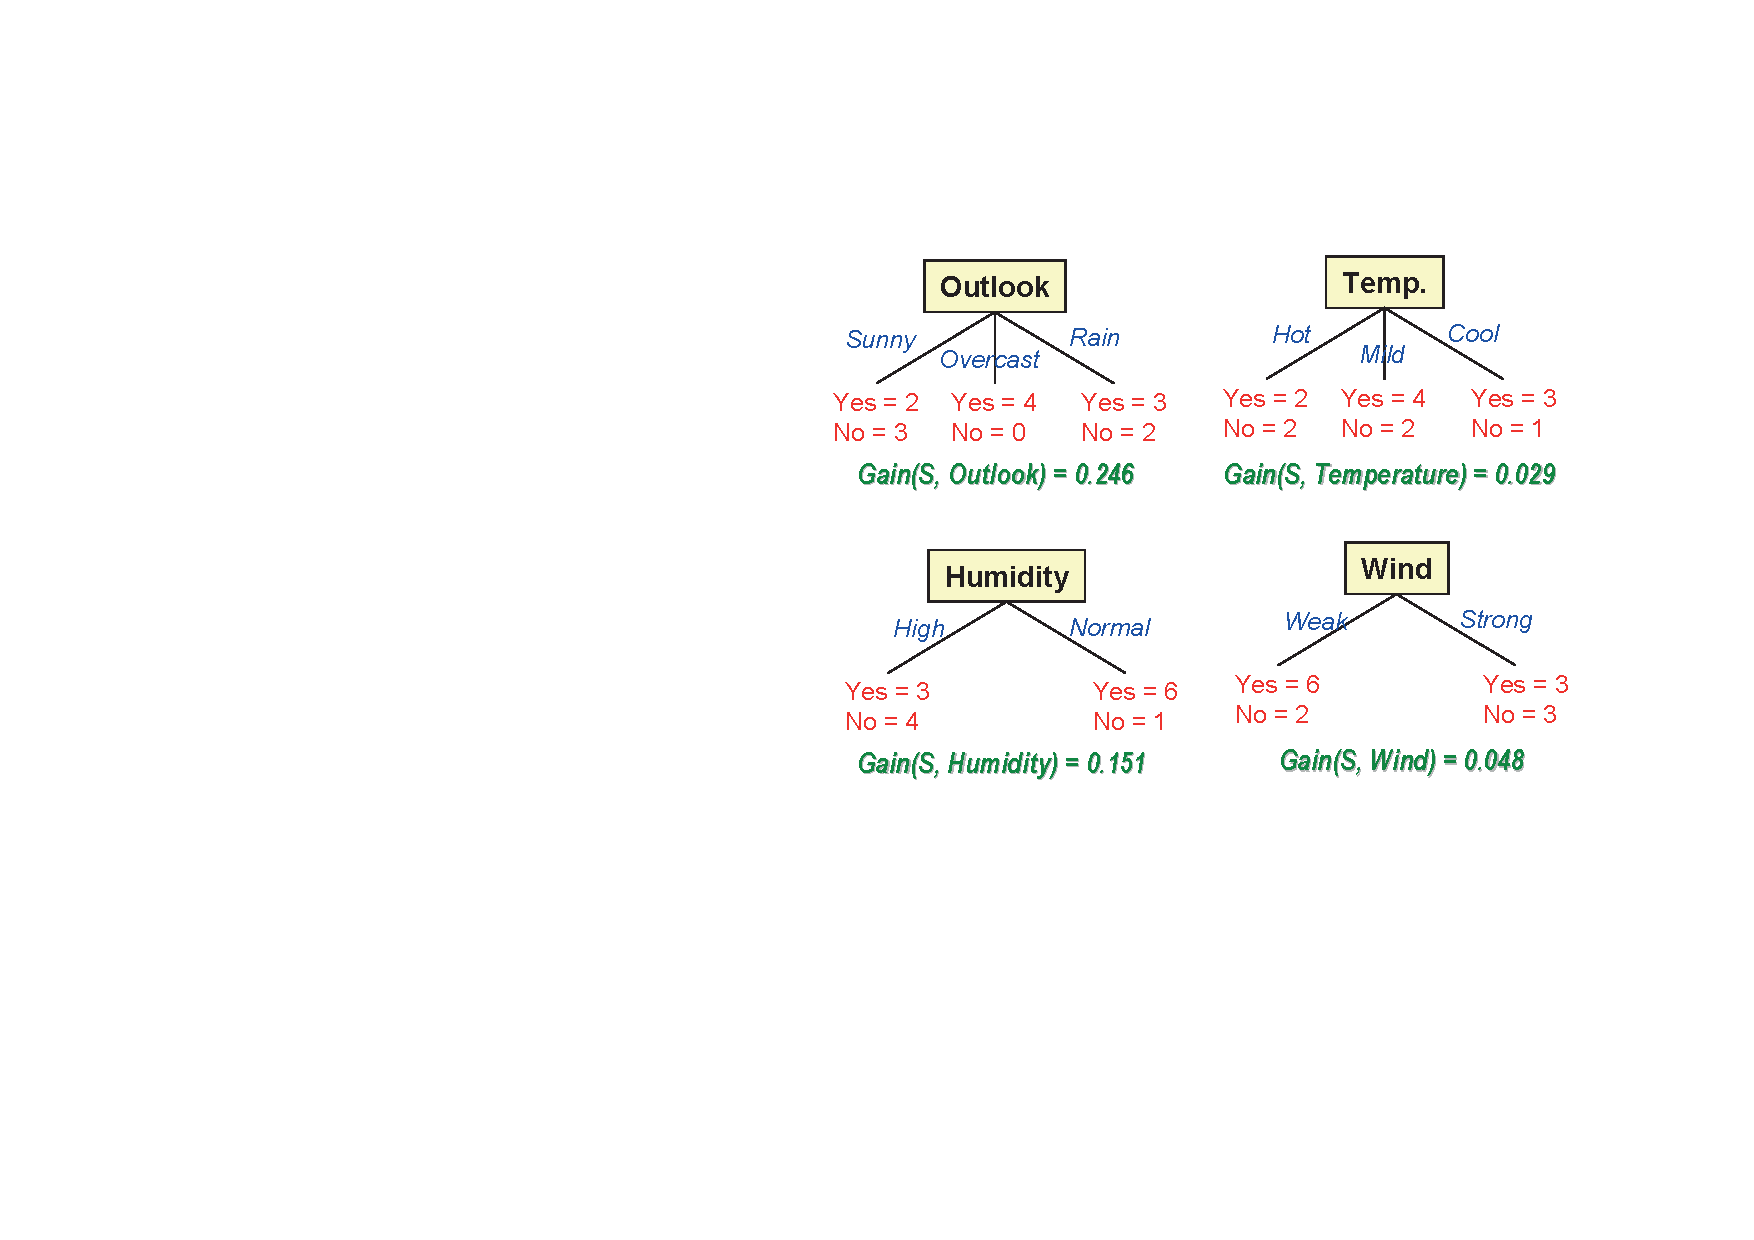
\includegraphics[width=0.80\textwidth]{tennis.pdf}
	\caption{根节点选择}
	\label{tennisnode}
\end{figure}

由于 Outlook 的信息增益最大, 所以应该选它作为根节点, 它将数据集$D$划分为 3 个分支,分别是 Sunny, Overcast 和 rain, 其中 Overcast 的分支只有同一类的样本点, 所以它成为一个叶节点, 节点的标记为“是”.


接下来我们要按照同样的办法对 Sunny 和 Rain 继续进行分支.

比如对 Sunny 进行分支, 为了方便观察, 我们将原始数据集中 Outlook = Sunny 的所有资料列出, 如下表:
\begin{table}[!htb]
\centering
\caption{网球数据}
\label{sunny}
\begin{tabular}{l|l|l|l|l|l}
  \hline
    % after \: \hline or \cline{col1-col2} \cline{col3-col4} ...
    \textbf{Day} & \textbf{Outlook} & \textbf{Temperature} & \textbf{Humidity} & \textbf{Wind} & \textbf{Play Tennis} \\
    \hline
    1 & Sunny & Hot & High & Weak & No \\ 
    \hline
    2 & Sunny & Hot & High & Strong  & No \\ 
    \hline
    8 & Sunny & Mild & High & Weak & No \\ 
    \hline
    9 & Sunny & Cool & Normal & Weak & Yes \\ 
    \hline
    11 & Sunny & Mild & Normal & Strong & Yes \\ 
  \hline
\end{tabular}
\end{table}

计算信息增益可得下图
\begin{figure}[!htb]
	\centering
	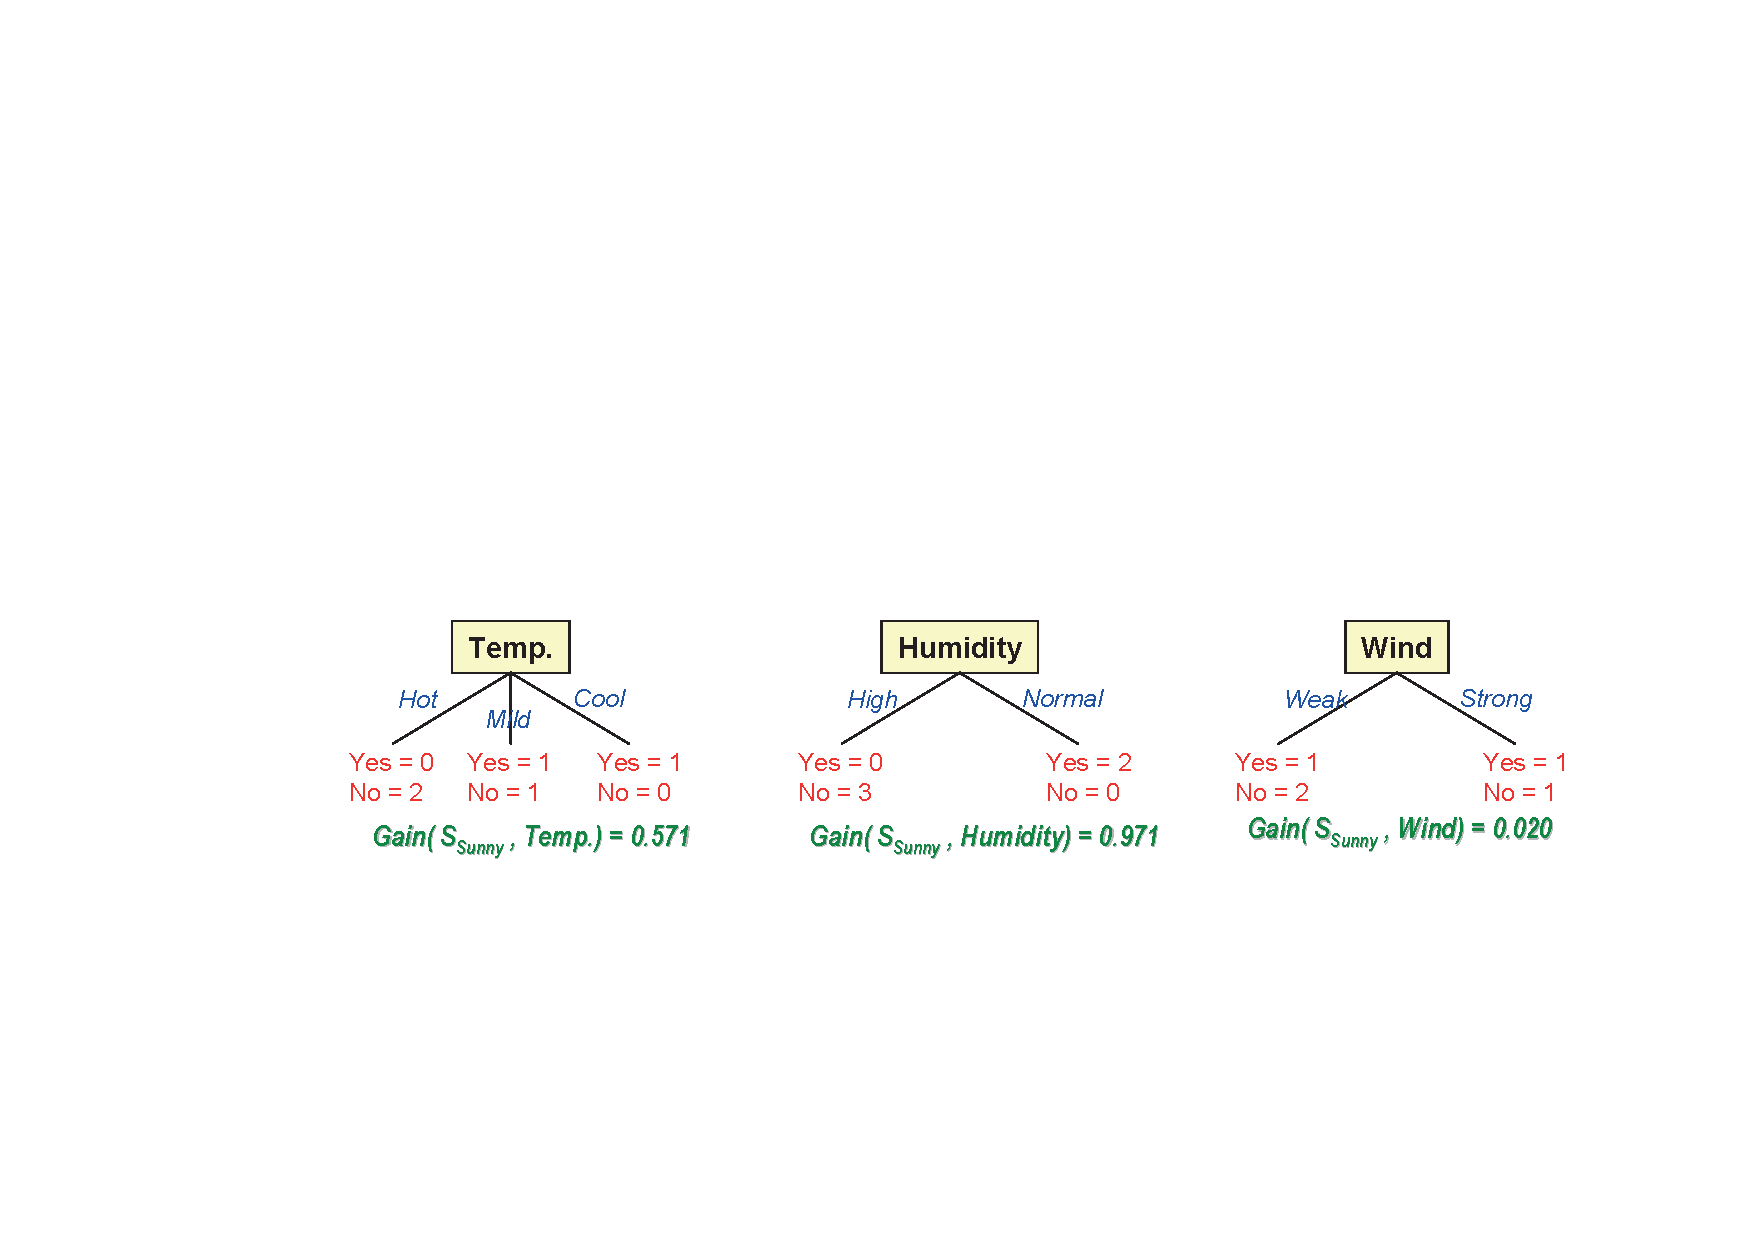
\includegraphics[width=0.85\textwidth]{sunny.pdf}
	\caption{Sunny分支}
	\label{sunnyfig}
\end{figure}


可以看到, 此时 Humidity 的信息增益最大, 故选取它为新节点, 它将 Sunny 分支划分为 2 个小分支, 分别是 Humidity = High 和 Humidity = Normal, 这两个小分支都是同一类的样本点, 所以它们成为 2 个叶节点, 节点的标记分为“是”和“否”.于是 Sunny 分支结束.

同理可对 Rain 分支进行讨论, 先把所有资料列出得下表
\begin{table}[!htb]
\centering
\caption{网球数据}
\label{rain}
\begin{tabular}{l|l|l|l|l|l}
  \hline
    % after \: \hline or \cline{col1-col2} \cline{col3-col4} ...
    \textbf{Day} & \textbf{Outlook} & \textbf{Temperature} & \textbf{Humidity} & \textbf{Wind} & \textbf{Play Tennis} \\
    \hline
    4 & Rain & Mild & High & Weak & Yes \\ 
    \hline
    5 & Rain & Cool & Normal & Weak & Yes \\ 
    \hline
    6 & Rain & Cool & Normal & Strong &  No \\ 
    \hline
    10 & Rain & Mild & Normal & Weak & Yes \\ 
    \hline
    14 & Rain & Mild & High & Strong & No \\ 
  \hline
\end{tabular}
\end{table}

同理计算可得(其实可直接看出来, 这里也就不再画图展示了), 此时 Wind 的信息增益最大, 它将 Rain 分支划分为 2 个小分支, 分别是 Wind = Weak 和 Wind = Strong, 这两个小分支都是同一类的样本点, 所以它们成为2个叶节点, 节点的标记分为“是”和“否”. 于是Rain分支结束.

综上可得决策树如下
\begin{figure}[!htb]
	\centering
	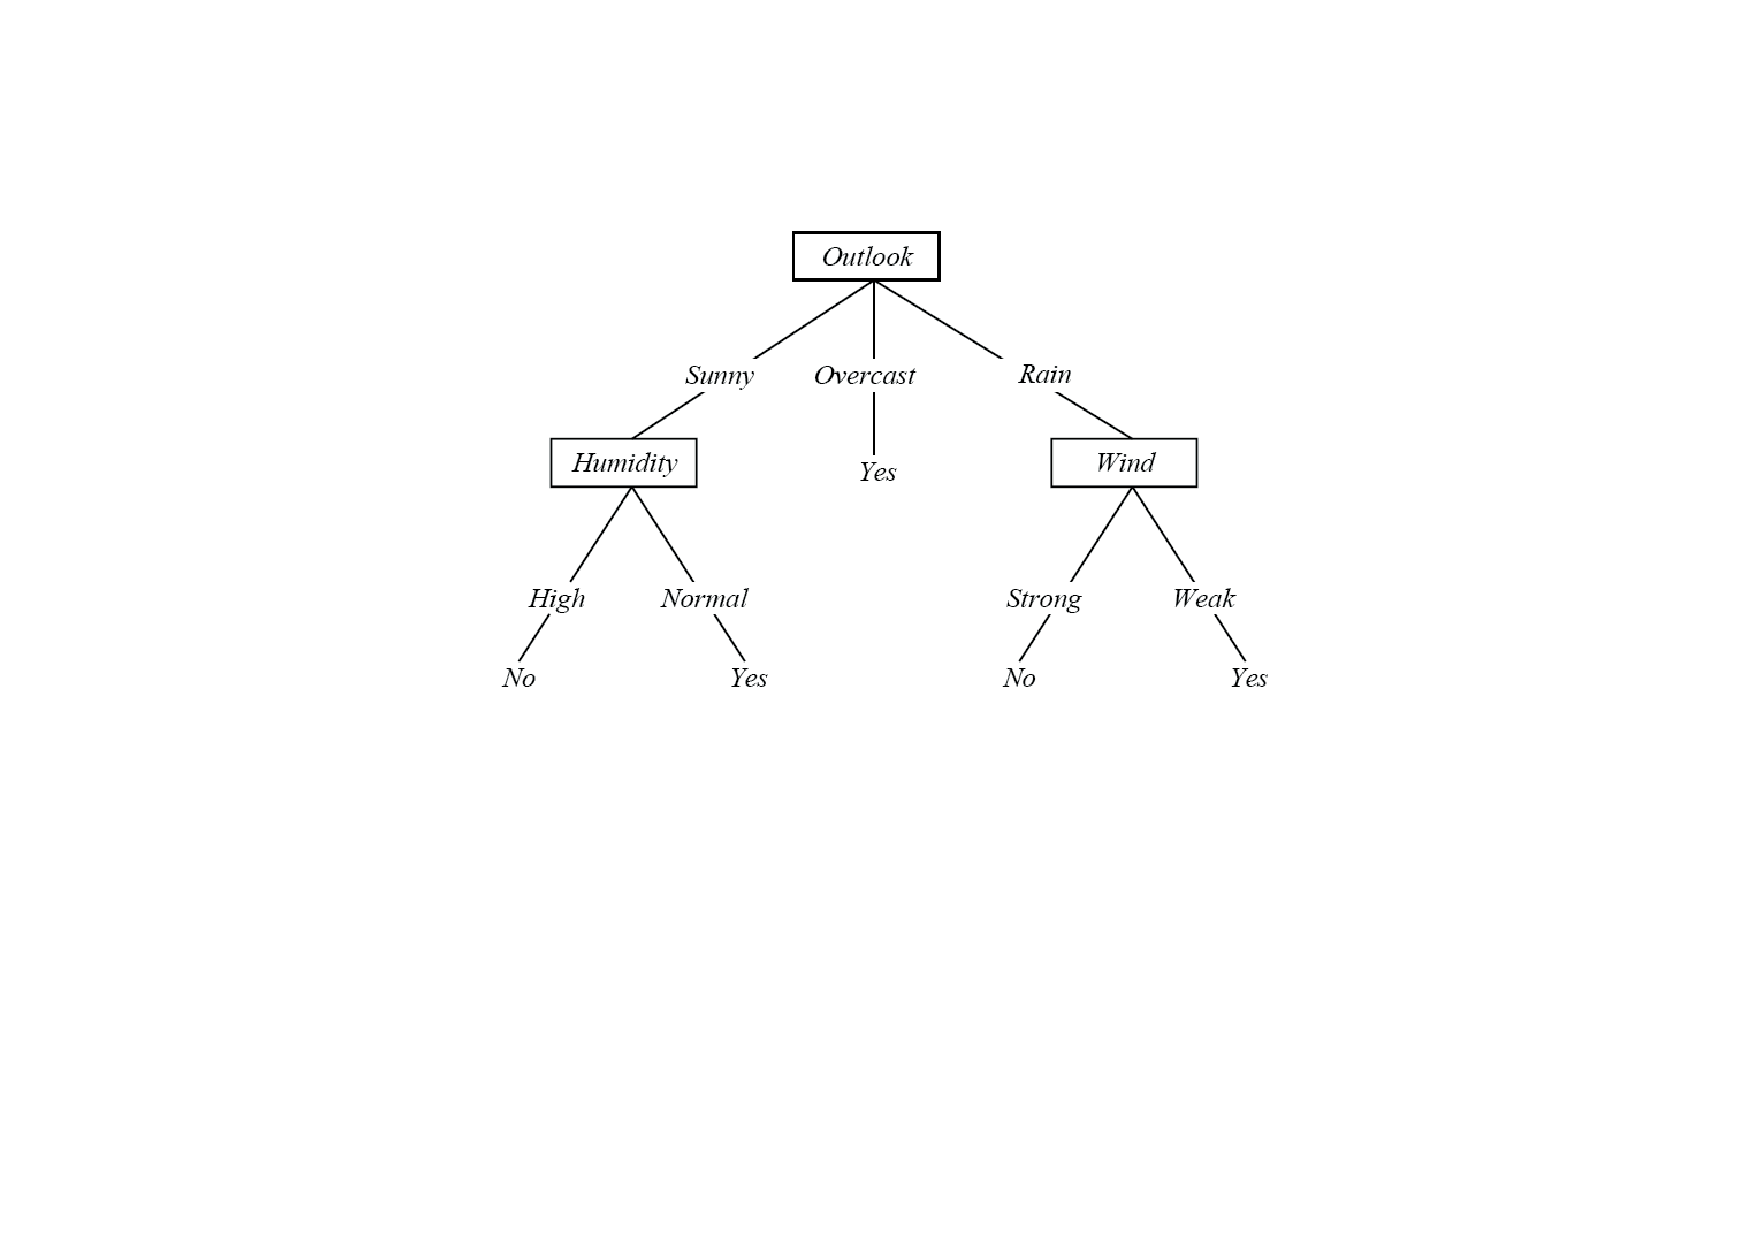
\includegraphics[width=0.80\textwidth]{table-tree.pdf}
	\caption{网球决策树}
	\label{tabletree}
\end{figure}

规则集如下
\begin{figure}[!htb]
	\centering
	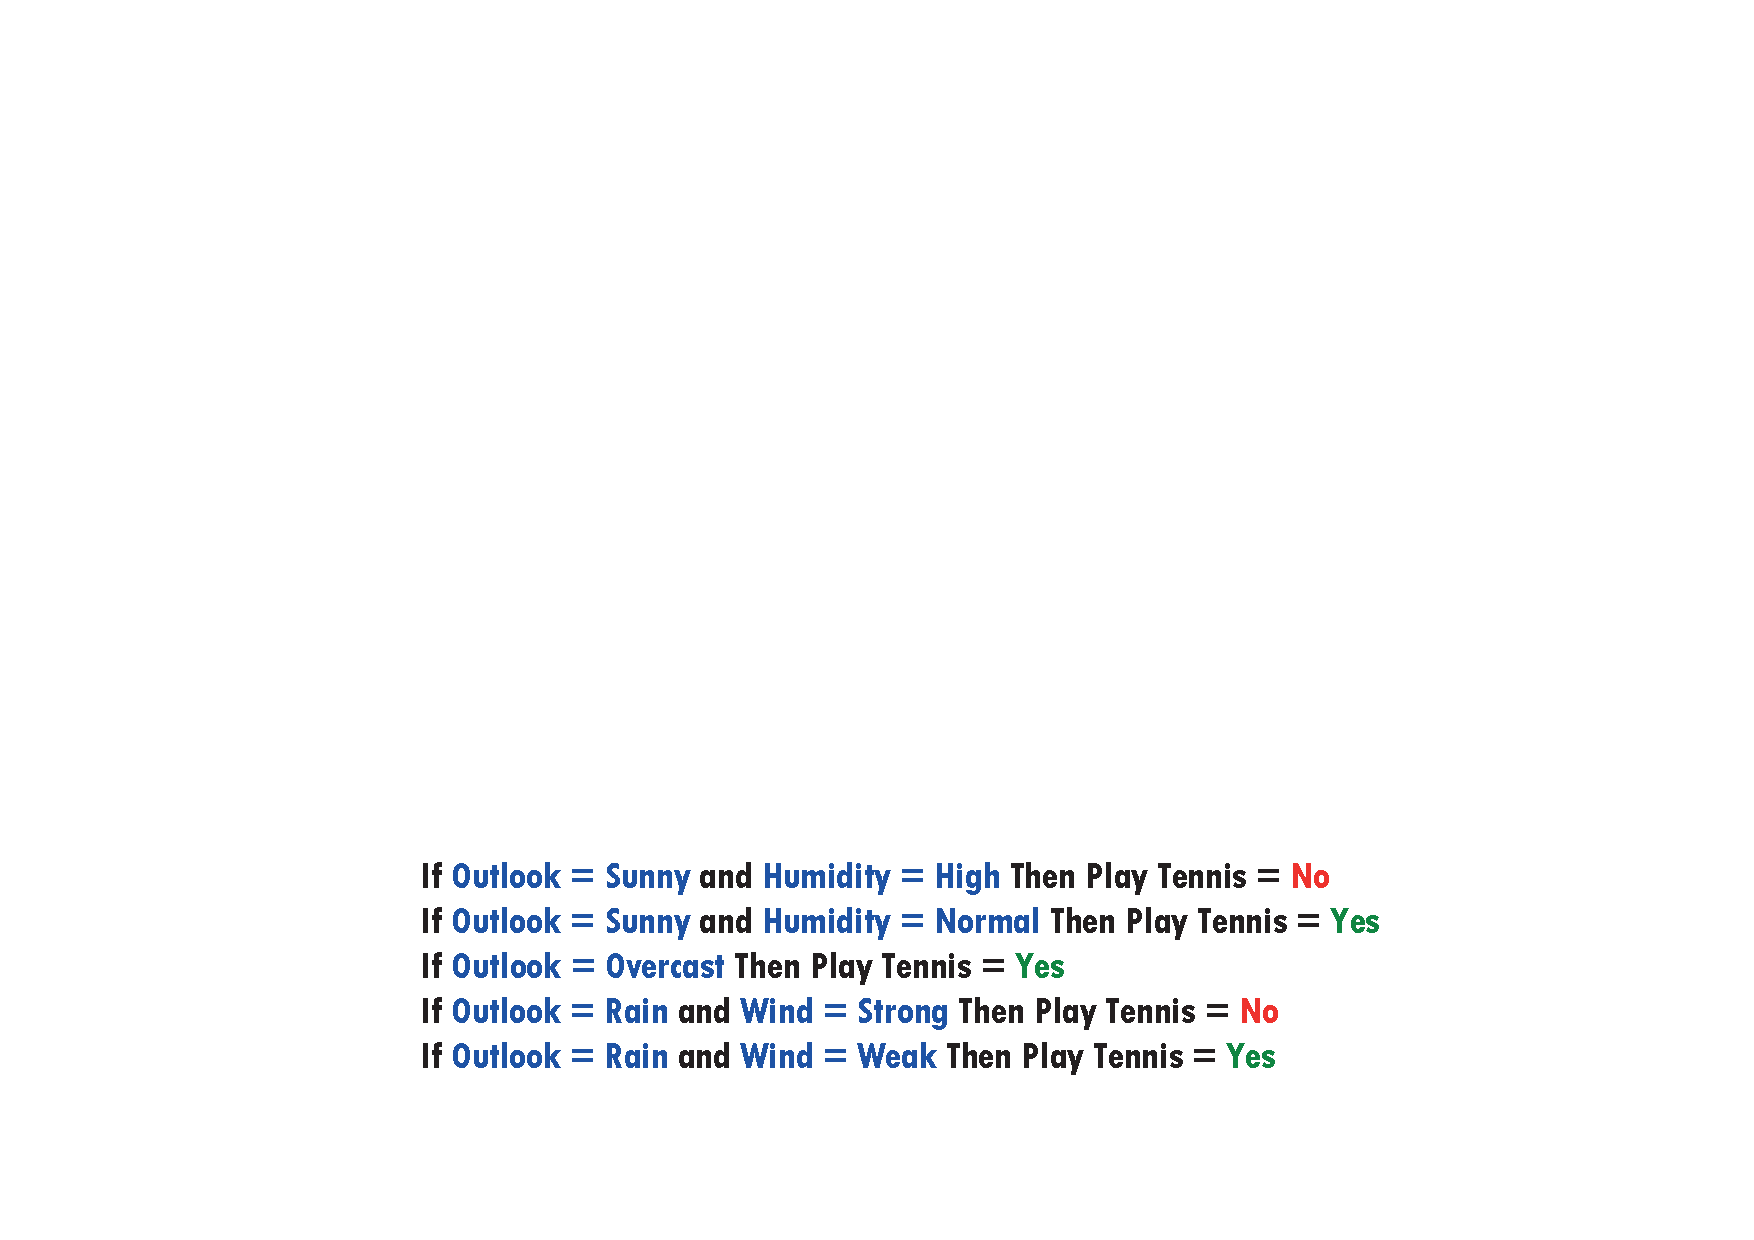
\includegraphics[width=0.85\textwidth]{table-rules}
	\caption{网球规则集}
	\label{tablerules}
\end{figure}




\subsection{打高尔夫的例子}
此例子来自维基百科.

小王是一家著名高尔夫俱乐部的经理, 但是他被雇员数量问题搞得心情十分不好. 某些天好像所有人都来玩高尔夫, 以至于所有员工都忙的团团转还是应付不过来, 而有些天不知道什么原因却一个人也不来, 俱乐部为雇员数量浪费了不少资金.

小王的目的是通过下周天气预报寻找什么时候人们会打高尔夫, 以适时调整雇员数量. 因此首先他必须了解人们决定是否打球的原因.

在 2 周时间内我们得到以下记录:
\begin{table}[!htb]
\centering
\caption{高尔夫数据}
\label{golf}
\begin{tabular}{c|c|c|c|c|c}
  \hline
    % after \: \hline or \cline{col1-col2} \cline{col3-col4} ...
    \textbf{Day} & \textbf{Outlook} & \textbf{Temperature} & \textbf{Humidity} & \textbf{Windy} & \textbf{Play Or Not} \\
    \hline
    1 & sunny & 85 & 85 & false & Don't Play \\ 
    \hline
    2 & sunny & 80 & 90 & true  & Don't Play \\ 
    \hline
    3 & overcast & 83 & 78 & false & Play \\ 
    \hline 
    4 & rain & 70 & 96 & false & Play \\ 
    \hline
    5 & rain & 68 & 80 & false & Play \\ 
    \hline
    6 & rain & 65 & 70 & true &  Don't Play \\ 
    \hline
    7 & overcast & 64 & 65 & true & Play \\ 
    \hline
    8 & sunny & 72 & 95 & false & Don't Play \\ 
    \hline
    9 & sunny & 69 & 70 & false & Play \\ 
    \hline
    10 & rain & 75 & 80 & false & Play \\ 
    \hline
    11 & sunny & 75 & 70 & true & Play \\ 
    \hline
    12 & overcast & 72 & 90 & true & Play \\ 
    \hline
    13 & overcast & 81 & 75 & false & Play \\
    \hline
    14 & rain & 71 & 80 & true & Don't Play \\ 
  \hline
\end{tabular}
\end{table}

其中 Outlook 表示天气类型, 天气状况有晴(sunny)、云(overcast、阴天)、和雨(rain); Temperature 表示温度, 气温用华氏温度表示; Humidity 表示湿度,相对湿度用百分比; Windy 表示有没有风. 当然还有顾客是不是在这些日子光顾俱乐部. 最终得到了 14 行 6 列的数据表格. 为了方便讨论, 我们将玩(Play)标记为正类, 将不玩(Don't Play)标记为负类.

显然数据集中有 9 个正类, 5 个负类, 因此该集合的信息熵为
\begin{equation*}
H(D) = - \frac{9}{14} \log \frac{9}{14} - \frac{5}{14} \log \frac{5}{14} = 0.940
\end{equation*}

我们仍用$A_i, i = 1, 2, 3, 4$表示样本的$4$个特征, 那么 Outlook 的信息增益为
\begin{align*}
g(D, A_{1}) & = H(D) - \left[ \frac{5}{14} H(D_{1}) + \frac{4}{14} H(D_{2}) + \frac{5}{14} H(D_{3}) \right] \\ 
& = 0.940 - \left[ \frac{5}{14} \left( - \frac{2}{5} \log \frac{2}{5} - \frac{3}{5} \log \frac{3}{5} \right) + \frac{4}{14} \times 0 + \frac{5}{14} \left( - \frac{3}{5} \log \frac{3}{5} - \frac{2}{5} \log \frac{2}{5} \right) \right] \\ 
& = 0.246
\end{align*}

此例子与上面的两个例子的不同之处在于某些特征是连续取值, 比如这里的气温和湿度, 而上面两个例子特征的取值都是离散的, 那我们该怎么做呢?

一个容易想到的方法是手动离散, 比如对于气温, 把它分为高温和低温两类, 高于$72.5$算高温, 低于$72.5$算低温, 当然也可以分为几个合适的区间, 这样就可以使用 ID3 算法了, 可是这里有个问题, 如何确定一个合理的界限呢?

以二分法为例, 我们来对气温排序, 如下
\begin{table}[!htb]
\centering
\caption{气温排序}
\label{temp}
\begin{tabular}{cccccccccccccc}
    \hline
    % after \: \hline or \cline{col1-col2} \cline{col3-col4} ...
    64 & 65 & 68 & 69 & 70 & 71 & 72 & 72 & 75 & 75 & 80 & 81 & 83 & 85 \\ 
    y  & n  & y  & y  & y  & n  & n  & y  & y  & y  & n  & y  & y  & n \\
    \hline
\end{tabular}
\end{table}

其中 y 表示 Play, n 表示Don't Play, 如果我们选用$71.5$为分隔点, 即小于$71.5$为低温, 那么低温中有 4 个正类, 2 个负类, 大于$71.5$为高温, 那么高温中有 5 个正类, 3 个负类, 那么此时特征 Temprature 的信息增益为
\begin{align*}
g(D, A_{2}) & = 0.940 - \left[ \frac{6}{14} \left( - \frac{4}{6} \log \frac{4}{6} - \frac{2}{6} \log \frac{2}{6} \right) + \frac{8}{14} \left( - \frac{5}{8} \log \frac{5}{8} - \frac{3}{8} \log \frac{3}{8} \right) \right] \\ 
& = 0.940 - 0.939 = 0.001
\end{align*}

当然, 我们也可以选其它的数作为分割点把特征 Temprature 分为两类计算它的信息增益, 我们可以遍历中间的所有值找到最优的分割点(具体可参考其它书籍), 然后计算 Temprature 的信息增益, 不过, 在高尔夫这个例子中, 仍然没有 Outlook 的信息增益大.

同理可计算 Himudity 和 Windy 的信息增益, 比较发现还是 Outlook 的信息增益大, 所以选 Outlook 为根节点, 然后分出$3$个枝节点, 其中 Overcast 为叶节点, 我们还需要对 Sunny 和 Rain 继续分支.

比如对 Sunny 进行分支, 先把表中 Sunny 的样本全都列出来
\begin{table}[!htb]
\centering
\caption{高尔夫数据}
\label{golfsunny}
\begin{tabular}{c|c|c|c|c|c}
  \hline
    % after \: \hline or \cline{col1-col2} \cline{col3-col4} ...
    \textbf{Day} & \textbf{Outlook} & \textbf{Temperature} & \textbf{Humidity} & \textbf{Windy} & \textbf{Play Or Not} \\
    \hline
    1 & sunny & 85 & 85 & false & Don't Play \\ 
    \hline
    2 & sunny & 80 & 90 & true  & Don't Play \\ 
    \hline
    8 & sunny & 72 & 95 & false & Don't Play \\ 
    \hline
    9 & sunny & 69 & 70 & false & Play \\ 
    \hline
    11 & sunny & 75 & 70 & true & Play \\ 
  \hline
\end{tabular}
\end{table}

接下来就不用计算了, 直接用肉眼去看即可, 显然用 Windy 属性没有办法把正负类完全区分开来, 那么 Temperature 和 Humdity 呢?

把 Temperature 排序, 如下表\ref{sunnytemp}
\begin{table}[!htb]
\centering
\caption{Sunny 下的 气温排序}
\label{sunnytemp}
\begin{tabular}{ccccc}
    \hline
    % after \: \hline or \cline{col1-col2} \cline{col3-col4} ...
    69  & 72  & 75  & 80  & 85  \\
    y   & n   & y   & n   & n  \\
    \hline
\end{tabular}
\end{table}

显然, 不管选哪个数作为分割点都无法将两类区分开.

再看 Humidity, 排序如下表\ref{sunnyhumi}
\begin{table}[!htb]
\centering
\caption{Sunny 下的 气温排序}
\label{sunnyhumi}
\begin{tabular}{ccccc}
    \hline
    % after \: \hline or \cline{col1-col2} \cline{col3-col4} ...
    70  & 70  & 85  & 90  & 95  \\
    y   & y   & n   & n   & n \\ 
    \hline
\end{tabular}
\end{table}

显然, 我们随便选一个$70$到$85$之间的数作为分割点都能把两类完全区分开, 比如就选$70$, 那么大于$70$的都是负类, 反之则是正类.

因此, Sunny 分支肯定选用 Humidity 为节点, 它的信息增益肯定也是最大的(选取$70$为分割点).

同理可以考察 Rain 分支, 把样本全部列出来, 见下表\ref{golfrain}
\begin{table}[!htb]
\centering
\caption{高尔夫数据}
\label{golfrain}
\begin{tabular}{c|c|c|c|c|c}
  \hline
    % after \: \hline or \cline{col1-col2} \cline{col3-col4} ...
    \textbf{Day} & \textbf{Outlook} & \textbf{Temperature} & \textbf{Humidity} & \textbf{Windy} & \textbf{Play Or Not} \\
    \hline
    4 & rain & 70 & 96 & false & Play \\ 
    \hline
    5 & rain & 68 & 80 & false & Play \\ 
    \hline
    6 & rain & 65 & 70 & true &  Don't Play \\ 
    \hline
    10 & rain & 75 & 80 & false & Play \\ 
    \hline
    14 & rain & 71 & 80 & true & Don't Play \\ 
  \hline
\end{tabular}
\end{table}

同理可直接看出 Windy 属性可直接将两类完全区分开来, 故选它作为分支节点即可, 事实上, 对这里的 Temperature 和 Humidity 数据排序, 会发现确实也找不到合适的分割点将两类完全区分开来.

最终生成的决策树如下图\ref{palygolf}
\begin{figure}[!htb]
    \centering
    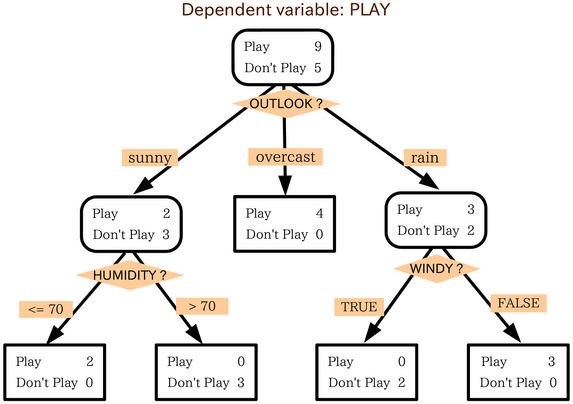
\includegraphics[width = 0.80 \textwidth]{play_golf.png}
    \caption{高尔夫决策树}
    \label{palygolf}
\end{figure}

图\ref{palygolf}是网上的, 我用 R 语言的 C50 包并没有生成这样的图(报错尚未解决), 倒是用 SPSS 的 Modeler 画出了类似的图, 如下图\ref{spss}.
\begin{figure}[!htb]
	\centering
	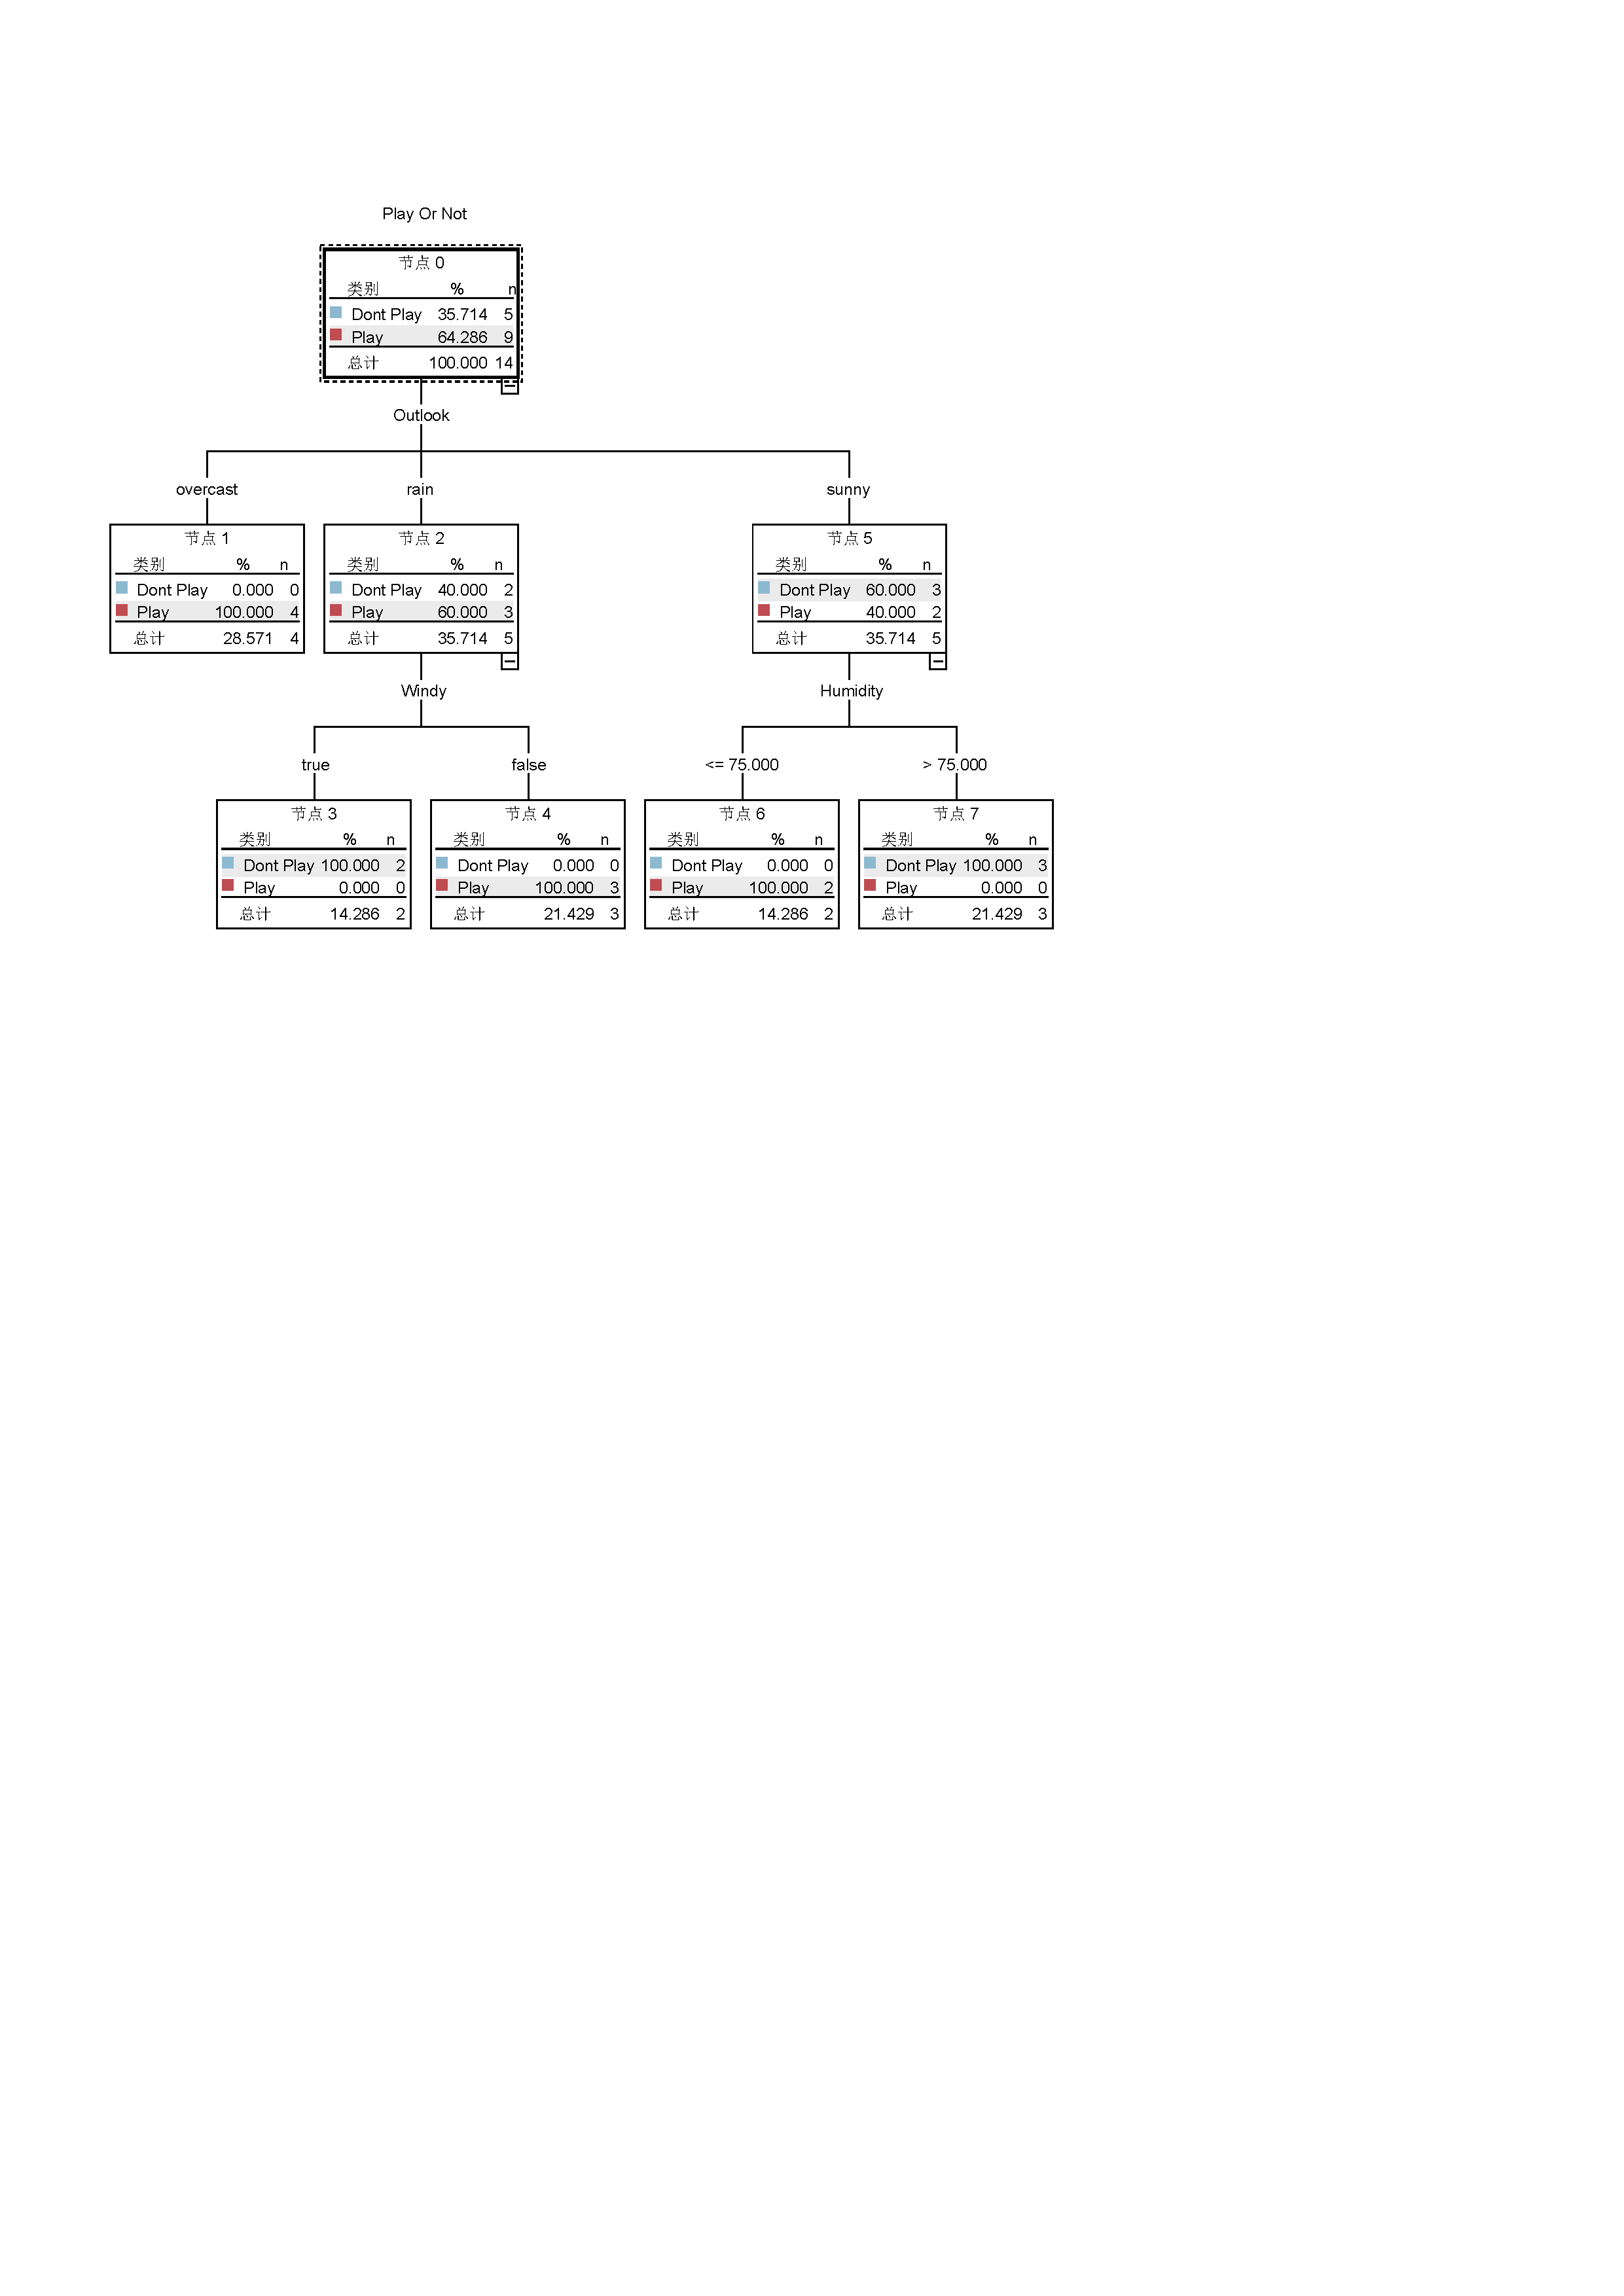
\includegraphics[width = 0.75 \textwidth]{golf.pdf}
	\caption{高尔夫决策树}
	\label{spss}
\end{figure}



\section{C4.5 算法和 C5.0 算法}
ID3 算法有很多不足, 上面已经提到特征连续取值的情形, 还有比如特征取值情况很多怎么办, 比如特征是日期, 这样如果使用 ID3 算法, 信息增益大的肯定倾向于选择取值多的特征作为分隔点, 为了避免类似的不足, 引入了 C4.5 算法, 它不是采用信息增益为分裂标准, 而是采用信息增益率(Information Gain Ratio)为分裂标准.

特征$A$对训练数据集$D$的信息增益比$g_{R}(D, A)$定义为其信息增益$g(D, A)$与训练数据集$D$的经验熵$H(D)$之比:
\begin{equation*}
g_{R}(D, A) = \frac{g(D, A)}{H(D)}
\end{equation*}

这是李航《统计学习方法》上的定义, 但我看大多数资料与之不同, 差别在分母上, 对于一个训练数据集$S$来说, 特征$A$的信息增益比定义为
\begin{equation*}
\mathrm{GainRatio}(S, A) = \frac{\mathrm{Gain(S, A)}}{\mathrm{SplitInformation}(S, A)}
\end{equation*}

其中$\mathrm{SplitInformation}(S, A)$称为分割信息值,
\begin{equation*}
\mathrm{SplitInformation}(S, A) = \sum_{i=1} \frac{|S_i|}{|S|} \log_{2} \frac{|S_i|}{|S|}
\end{equation*}

以前面第二个例子, 也就是打网球那个例子为例, 比如要计算特征“Wind”的信息增益率, 由前面我们已经算出
\begin{equation*}
\mathrm{Gain}(S, \mathrm{Wind}) = 0.048
\end{equation*}

而“Windy”中有 8 个“false”, 6 个“true”, 因此其分割信息值为
\begin{equation*}
\mathrm{SplitInfo}(S, \mathrm{Wind}) = -\frac{8}{14} \times \log_{2} \frac{8}{14} - \frac{6}{14} \times \log_{2} \frac{6}{14} = 0.985
\end{equation*}

因此“Wind”的信息增益率为
\begin{equation*}
\mathrm{GainRation}(S, \mathrm{Wind}) = \frac{0.048}{0.985} = 0.049
\end{equation*}

同理可得其它三个的信息增益率
\begin{itemize}
\item Outlook: Gain(S, Outlook) = 0.246, SplitInfo = 1.577, GainRation = 0.156

\item Temp: Gain(S,Temp) = 0.029,  SplitInfo = 1.362, GainRation = 0.021

\item Humidity: Gain(S,Humidity) = 0.151,  SplitInfo = 1, GainRation = 0.151
\end{itemize}

可以看出, 对于本例子, 如果采用信息增益率为分裂标准, 使用 Outlook 仍然是最好的, 但是现在 Humidity 成了有力的竞争者.

后续的过程可以同理计算, 这里就不再多述了.


C5.0 是 C4.5 的商业改进版, 可应用于海量资料集合上之分类, 主要在执行准确度和内存占用方面做了改进, 因其采用 Boosting 方式来提高准确率, 且占用系统资源少, 所以计算速度较快. C5.0 算法依照最大信息增益的概念来切割样本, 并重复进行切割直到样本子集不能再被分割为止.

R 语言有 C5.0 包可以进行C5.0决策树的建模分析, 其介绍可见\url{http://www.rulequest.com/see5-unix.html}.




\section{过拟合与正则化}
同其他分类算法一样, 决策树模型也会产生过拟合, 这是一个很重要的问题.决策树里面通过剪枝操作来避免过拟合.










\section{CART 算法}
分类与回归树(Clasification And Regression Tree, CART) 模型也是一个应用广泛的决策树学习方法. 这里我们先讨论分类.

CART 与 ID3、C4.5、C5.0 算法的最大不同之处是其在每一个节点上采用的是二分法, 也就是一次只能够有两个子节点, ID3、C4.5、C5.0 则在每一个节点上可以产生多个不同的分支. 除此之外, CART 选用基尼(Gini)系数来作为选择属性的标准.

分类问题中, 假设有$K$个类, 样本点属于第$k$类的概率为$p_{k}$, 则概率分布的基尼指数定义为
\begin{equation*}
\mathrm{Gini}(p) = \sum_{i=1}^{K} p_{k} (1 - p_{k}) = 1 - \sum_{k=1}^{K} p_{k}^{2}
\end{equation*}

特别的, 对于二分类问题, 若样本点属于第1个类(正类)的概率是$p$, 则概率分布的基尼指数为
\begin{equation*}
\mathrm{Gini}(D) = 2p(1-p)
\end{equation*}

对于给定的样本集合$D$, 其基尼指数为
\begin{equation*}
\mathrm{Gini}(D) = 1 - \sum_{k=1}^{K} \left( \frac{|C_k|}{|D|} \right)^2
\end{equation*}

其中$C_k$是$D$中属于第$k$类的样本子集, $K$是类的个数.

如果样本集合$D$根据特征$A$是否取某一可能值$a$被分割成$D_{1}$和$D_{2}$两部分,则在特征$A$的条件下, 集合$D$的基尼指数定义为
\begin{equation*}
\mathrm{Gini}(D, A) = \frac{|D_1|}{|D|} \mathrm{Gini}(D_1) + \frac{|D_2|}{|D|} \mathrm{Gini}(D_2)
\end{equation*}

基尼指数$\mathrm{Gini}(D)$表示集合$D$的不确定性, 基尼指数$\mathrm{Gini}(D,A)$表示经$A = a$分割后集合$D$的不确定性. 基尼指数值越大, 样本集合的不确定性也就越大, 这一点与熵相似.

下面我们以第一个例子也就是信贷那个例子为例, 来说明 CART 的算法.

首先计算各特征的基尼指数, 选择最优特征以及最优切分点.仍然采用前面的记号, 分别以$A_1,A_2,A_3,A_4$表示年龄、有工作、有自己的房子和信贷情况$4$个特征, 然后用具体的数值区分特征的不同取值, 比如这里用$1,2,3$表示年龄的值青年、中年和老年, 以$1,2$表示有工作和有自己的房子的值为是和否, 以$1,2,3$表示信贷情况的值为非常好、好和一般.

先来求特征$A_{1}$的基尼指数, $A_1$有$3$个可能取值, 我们说过 CART 采用的是二分法, 所以我们要将其组合起来分为两类, 比如分为青年和非青年, 或者分为中年和非中年, 或者分为老年和非老年, 这三种情况我们都要讨论, 比如分为青年和非青年, 青年有$5$人(2 个正类, 3 个负类), 非青年有$10$人(7 个正类, 3 个负类), 因此
\begin{align*}
\mathrm{Gini}(D, A_{1} = 1) = \frac{5}{15} \left( 2 \times \frac{2}{5} \times \left( 1 - \frac{2}{5} \right) \right) + \frac{10}{15} \left( 2 \times \frac{7}{10} \times \left( 1 - \frac{7}{10} \right) \right) = 0.44
\end{align*}

同理可得
\begin{equation*}
\mathrm{Gini}(D, A_{1} = 2) = 0.48, \mathrm{Gini}(D, A_{1} = 3) = 0.44
\end{equation*}

由于$\mathrm{Gini}(D, A_{1} = 1)$和$\mathrm{Gini}(D, A_{1} = 3)$相等, 都是最小, 所以$A_{1} = 1$和$A_{1} = 3$都可以选作$A_{1}$的最优切分点.

再来求特征$A_{2}$和$A_{3}$的基尼指数, 由于它们都只有两个取值, 就不用再自己组合了, 直接简记为$\mathrm{Gini}(D, A_2)$和$\mathrm{Gini}(D, A_3)$, 计算可得
\begin{equation*}
\mathrm{Gini}(D, A_2) = 0.32, \mathrm{Gini}(D, A_3) = 0.27
\end{equation*}

由于$A_2$和$A_3$都只有一个切分点, 所以它们就是最优切分点.

再求特征$A_4$的基尼指数, 跟$A_{1}$一样, 它也有$3$中取值, 所以也有$3$种组合, 计算可得
\begin{equation*}
\mathrm{Gini}(D, A_{4} = 1) = 0.36, \mathrm{Gini}(D, A_{4} = 2) = 0.47, \mathrm{Gini}(D, A_{4} = 3) = 0.32
\end{equation*}

其中$\mathrm{Gini}(D, A_{4} = 3)$最小, 所以$A_{4} = 3$为$A_4$的最优切分点.

在$A_1, A_2, A_3, A_4$这几个特征中, $\mathrm{Gini}(D, A_{3}) = 0.27$最小, 所以选择特征$A_{3}$为最优特征, $A_{3} = 1$为最优切分点. 于是根节点生成两个子节点, 一个是叶节点. 对另一个节点继续使用以上方法在$A_1, A_2, A_4$中选择最优特征及其最优切分点, 结果是$A_{2} = 1$, 依次计算得知, 所得节点都是叶节点.

对于信贷这个例子, 按照 CART 算法所生成的决策树和 ID3 算法一样, 可见\ref{xindaitree}.

我们也可以看第二个例子, 也就是打网球那个例子, 集合$S$中有$9$个正类, $5$个负类, 因此该集合的基尼系数$\mathrm{Gini}(S)$为
\begin{equation*}
\mathrm{Gini}(S) = 2 \times \frac{9}{14} \times \left( 1 - \frac{9}{14} \right) \left( = 1 - \left( \frac{9}{14} \right)^2 - \left( \frac{5}{14} \right)^2 \right) = 0.459
\end{equation*}

然后开始看属性 Outlook, 这里也有$3$中组合, 为了举例, 我们只算一种组合, 即分为 Overcast (有$4$个) 和非 Overcast(有$10$个, 把 Sunny 和 Rain 归为一类), 可得
\begin{equation*}
\mathrm{Gini}(D, \mathrm{Outlook}) = \frac{10}{14} \left( 2 \times \frac{5}{10} \times \left( 1 - \frac{5}{10} \right) \right) + \frac{4}{14} \left( 2 \times \frac{4}{4} \times \left( 1 - \frac{4}{4} \right) \right) = 0.3571
\end{equation*}

同理, 对于Temprature, 不妨分为 Mild (6 个)和非 Mild(8 个, 把 Hot 和 Cool 合到一块), 计算可得
\begin{equation*}
\mathrm{Gini}(D, \mathrm{Temp}) = \frac{8}{14} \left( 2 \times \frac{5}{8} \times \frac{3}{8} \right) + \frac{6}{14} \left( 2 \times \frac{4}{6} \times \frac{2}{6} \right) = 0.458
\end{equation*}

对于 Humidity, 只有 High(7 个) 和 Normal(7 个), 因此可得
\begin{equation*}
\mathrm{Gini}(D, \mathrm{Humidity}) = \frac{7}{14} \left( 2 \times \frac{3}{7} \times \frac{4}{7} \right) + \frac{7}{14} \left( 2 \times \frac{6}{7} \times \frac{1}{7} \right) = 0.37
\end{equation*}

对于 Wind, 只有 Weak (8 个) 和  Strong (6 个), 因此可得
\begin{equation*}
\mathrm{Gini}(D, \mathrm{Wind}) = \frac{8}{14} \left( 2 \times \frac{6}{8} \times \frac{2}{8} \right) + \frac{6}{14} \left( 2 \times \frac{3}{6} \times \frac{3}{6} \right) = 0.43
\end{equation*}

由此可知, Outlook 具有最小的基尼系数(为$0.3571$), 故选它作为根节点, 后面的分支可同样计算, 这里不再多述.


\section{关于决策树的补充}
\subsection{决策树用于回归}
决策树也可用于回归, 比如拟合正弦函数, 如下图\ref{regressiontree}, 代码来自 \url{http://scikit-learn.org/stable/auto_examples/tree/plot_tree_regression.html#example-tree-plot-tree-regression-py}, 可见附录.
\begin{figure}[!htb]
    \centering
    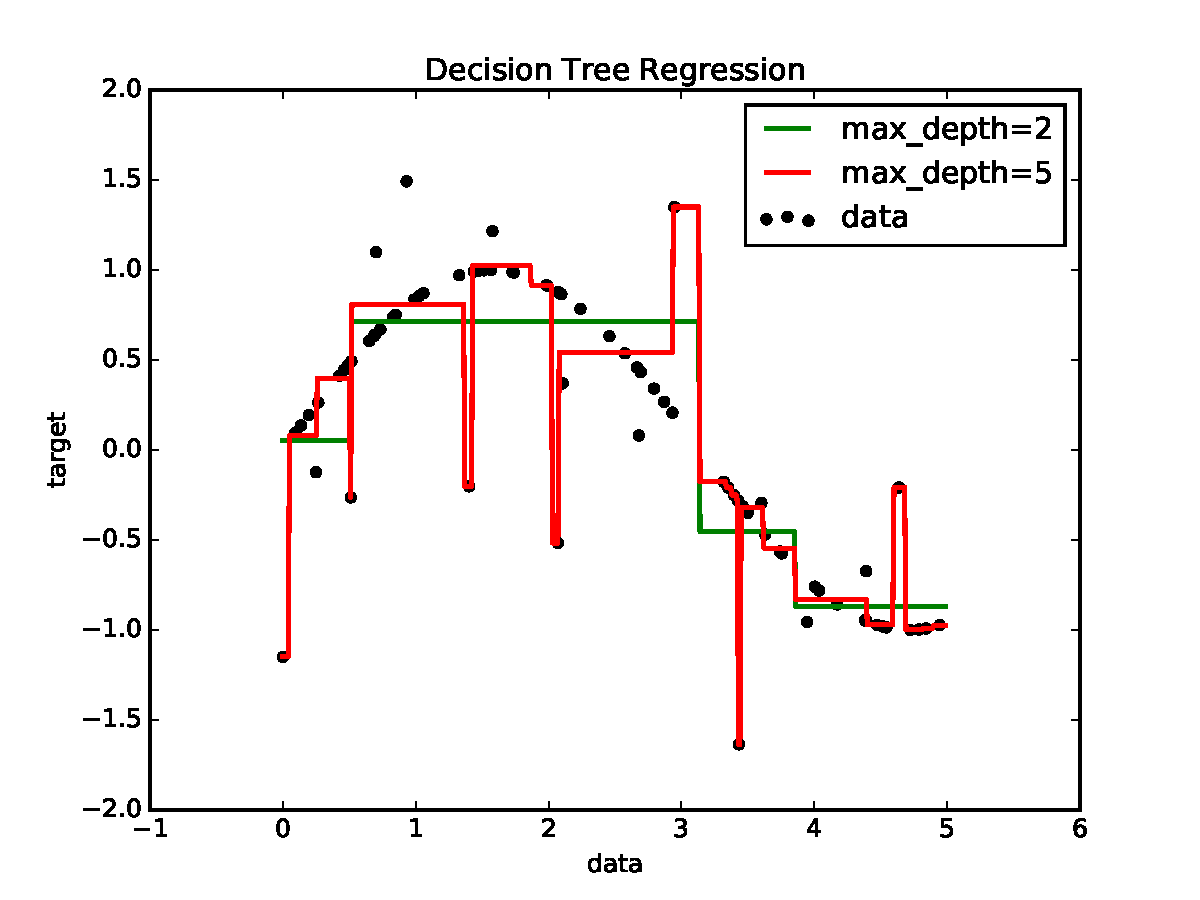
\includegraphics[width = 0.75 \textwidth]{regression_tree.pdf}
    \caption{回归决策树}
    \label{regressiontree}
\end{figure}


\subsection{决策树中的其它重要参数}




\section{总结}
\subsection{参考资料}
\begin{enumerate}[(1)]
\item 李航的《统计学习方法》, 不再多说.

\item 台湾陈士杰的决策树学习课件, 讲的比较清楚

\item 博客, 可见 \url{http://leijun00.github.io/datamining/}, 里面基本算是李航《统计学习方法》的 copy 版本.

\end{enumerate}



\subsection{决策树模型的应用场景}





\subsection{决策树模型的优缺点}





\newpage

\section*{附录}

回归树代码:
\begin{lstlisting}[language = python]
import numpy as np
from sklearn.tree import DecisionTreeRegressor
import matplotlib.pyplot as plt

# Create a random dataset
rng = np.random.RandomState(1)
X = np.sort(5 * rng.rand(80, 1), axis=0)
y = np.sin(X).ravel()
y[::5] += 3 * (0.5 - rng.rand(16))

# Fit regression model
regr_1 = DecisionTreeRegressor(max_depth=2)
regr_2 = DecisionTreeRegressor(max_depth=5)
regr_1.fit(X, y)
regr_2.fit(X, y)

# Predict
X_test = np.arange(0.0, 5.0, 0.01)[:, np.newaxis]
y_1 = regr_1.predict(X_test)
y_2 = regr_2.predict(X_test)

# Plot the results
plt.figure()
plt.scatter(X, y, c="k", label="data")
plt.plot(X_test, y_1, c="g", label="max_depth=2", linewidth=2)
plt.plot(X_test, y_2, c="r", label="max_depth=5", linewidth=2)
plt.xlabel("data")
plt.ylabel("target")
plt.title("Decision Tree Regression")
plt.legend()
plt.show()
\end{lstlisting}









\end{document}